\clearpage
\section{Motorcontroller}

The chassis used for the rover has 4 pre-installed DC motors, which are used for movement. To control the direction of the rover a Sabertooth 2x5 motor controller has been connected to the motors. The motor controller is used to operate the steering, forward and reversing actions of the rover.

\begin{figure}[H]
	\centering
	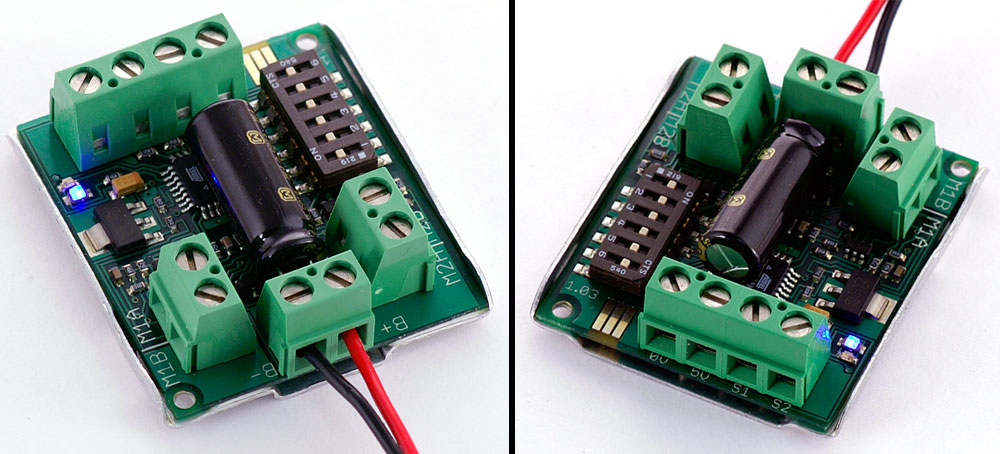
\includegraphics[width=.8\linewidth]{images/Sabertooth2X5big.jpg}
	\caption{Sabertooth 2x5\cite{sabertoothpic}}
\end{figure}

The driver uses a 5V supply to operate, which is easily supplied by the Raspberry Pi that is used to control the entire rover. The board supports two separate DC motor outputs that can independently controlled, in this case two motors will be connected to either side.

The dipswitches on the motor controller enables many different configuration options. For this project the controller will be set to analog mode, this means that the motor controllers logic level 0 is at 2.5V with the range 0V-5V. If the input voltage is above 2.5V it will generate a forward motion and if the signal is below 2.5V there will instead be generated a backwards motion. Since this particular motor controller has two signal inputs, it is possible to control two different directions\cite{sabertoothdata}.

Since the GPIO pins on a raspberry pi are rated at 3.3V will be using the controller in 4x sensitivity mode also. This changes the logic level range from 0V-5V with zero at 2.5V, to a logic range of 1.875V-3.125V with zero at 2.5V.  
This makes the controller more compatible with the raspberry pi.

The Raspberry has no analog outputs, therefore to obtain the necessary signals to control the motors PWM (Pulse width modulation) will is used. Using the following calculations the length of the duty-cycles was determined,

$3.3V(\frac{zero_v}{100}) = 2.5V\quad zero_v = 75.75\%$ \\
$3.3V(\frac{forward_v}{100}) = 3.125V\quad forward_v = 94.69\%$ \\
$3.3V(\frac{reverse_v}{100}) = 1.875V\quad reverse_v = 56.81\%$ \\



%Talk about how the signalling works
%Possibly add a diagram

%http://www.dimensionengineering.com/datasheets/Sabertooth2X5QuickStart.pdf
%http://www.dimensionengineering.com/datasheets/Sabertooth2x5.pdf
%http://www.dimensionengineering.com/products/sabertooth2x5